\documentclass[tikz,border=5pt]{standalone}
\usepackage{tikz}
\usetikzlibrary{arrows.meta}
\definecolor{nebula}{HTML}{6366F1}
\definecolor{spark}{HTML}{14B8A6}
\definecolor{ink}{HTML}{334155}
\begin{document}
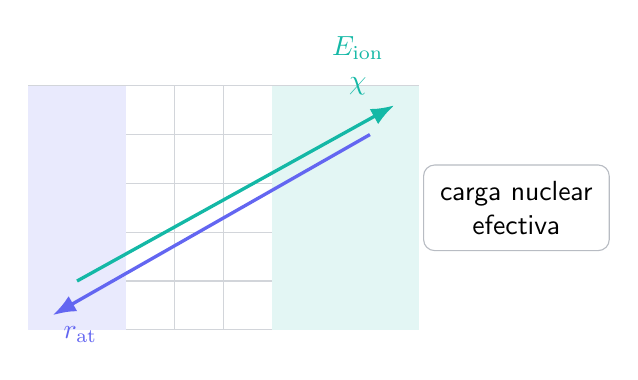
\begin{tikzpicture}[font=\sffamily,>=Latex,x=.62cm,y=.62cm]
  \foreach \x in {0,...,7} {\foreach \y in {0,...,4} {\draw[ink!22] (\x,\y) rectangle ++(1,1);}}
  \fill[nebula!14] (0,0) rectangle (2,5);
  \fill[spark!12] (5,0) rectangle (8,5);
  \draw[->,very thick,spark] (1,1)--(7.5,4.6) node[above left,align=center] {$E_{\rm ion}$\\$\chi$};
  \draw[->,very thick,nebula] (7,4)--(.5,.3) node[below right,align=center] {$r_{\rm at}$};
  \node[draw=ink!35,rounded corners=4pt,fill=white,inner sep=6pt,align=center]
    at (10,2.5) {carga nuclear\\efectiva};
\end{tikzpicture}
\end{document}
